\chapter{Theoretischer Hintergrund}
\label{sec:ThHi:first}

In diesem Kapitel soll die Theorie rund um IoT-Lösungen mit Funktechnologien behandelt werden. Anfangs werden bisher typische Protokolle und deren Netzwerkarchitekturen analysiert und verglichen. Daraufhin wird intensiv auf LoRa und LoRaWAN eingegangen. 

\section{Typische IoT-Protokolle}
\label{sec:ThHi:typical}

IoT-Lösungen spannen stets ein Netzwerk aus Geräten wie Sensoren und Aktoren auf. Derartige Netzwerke unterscheiden sich primär in den Eigenschaften Kosten, Reichweite, Energieverbrauch und Bandbreite. Diese Arbeit beschäftigt sich hierbei ausschließlich mit Funktechnologien. Für Szenarien wie Smart Buildings, Smart Cities oder ähnliches können die verwendeten Protokolle größtenteils in die Klassen \Begriff{WPAN} (Wireless Private Area Network) und \Begriff{LPWAN} (Low-power wide-area network) eingeordnet werden. Aus beiden Klassen werden nun Protokolle detailliert beschrieben, um anschließend ein besseres Verständnis darüber erlangen zu können, in welcher Sparte sich LoRa befindet. Hierbei gilt es zu beachten, dass die meisten IoT-Protokolle mehrere Schichten des allgemein bekannten TCP/IP-Schichtenmodells ausmachen und daher nicht nur die Datenübertragung selbst, sondern auch wichtige Aspekte wie beispielsweise die Netzwerkstruktur festlegen.

\subsection{Wireless Private Area Networks}
\label{sec:ThHi:pan}

Wie der Name bereits verrät, handelt es sich bei WPANs um Netzwerke, die für den drahtlosen Datenaustausch zwischen privaten Geräten genutzt werden. Die Protokolle dieser Klasse unterstützen typischerweise verhältnismäßig höhere Bandbreiten, wodurch jedoch die Reichweite stark leidet. Viele der, in der Vergangenheit meist für IoT verwendeten, Protokolle finden sich in der Klasse WPAN. In diesem Abschnitt werden die Protokolle \Fachbegriff{Zigbee} und \Fachbegriff{Bluetooth Low Energy} behandelt.

\subsubsection{Zigbee}
\label{sec:ThHi:Zigbee}

Zigbee ist bis heute eines der beliebtesten Protokolle für IoT-Lösungen. Gerade durch die Einfachheit des Protokolls und der Netzwerkstruktur ist Zigbee in Smart Homes und ähnlichen Szenarien sehr beliebt. Das Protokoll wird von der Zigbee Alliance entwickelt und verwaltet. Neben dem bidirektionalen Versand bietet Zigbee Funktionen wie zum Beispiel eine AES-Verschlüsselung in der Netzwerk- und der Anwendungsschicht. 

\begin{figure}[H]
  \vspace{10pt}
  \begin{center}
    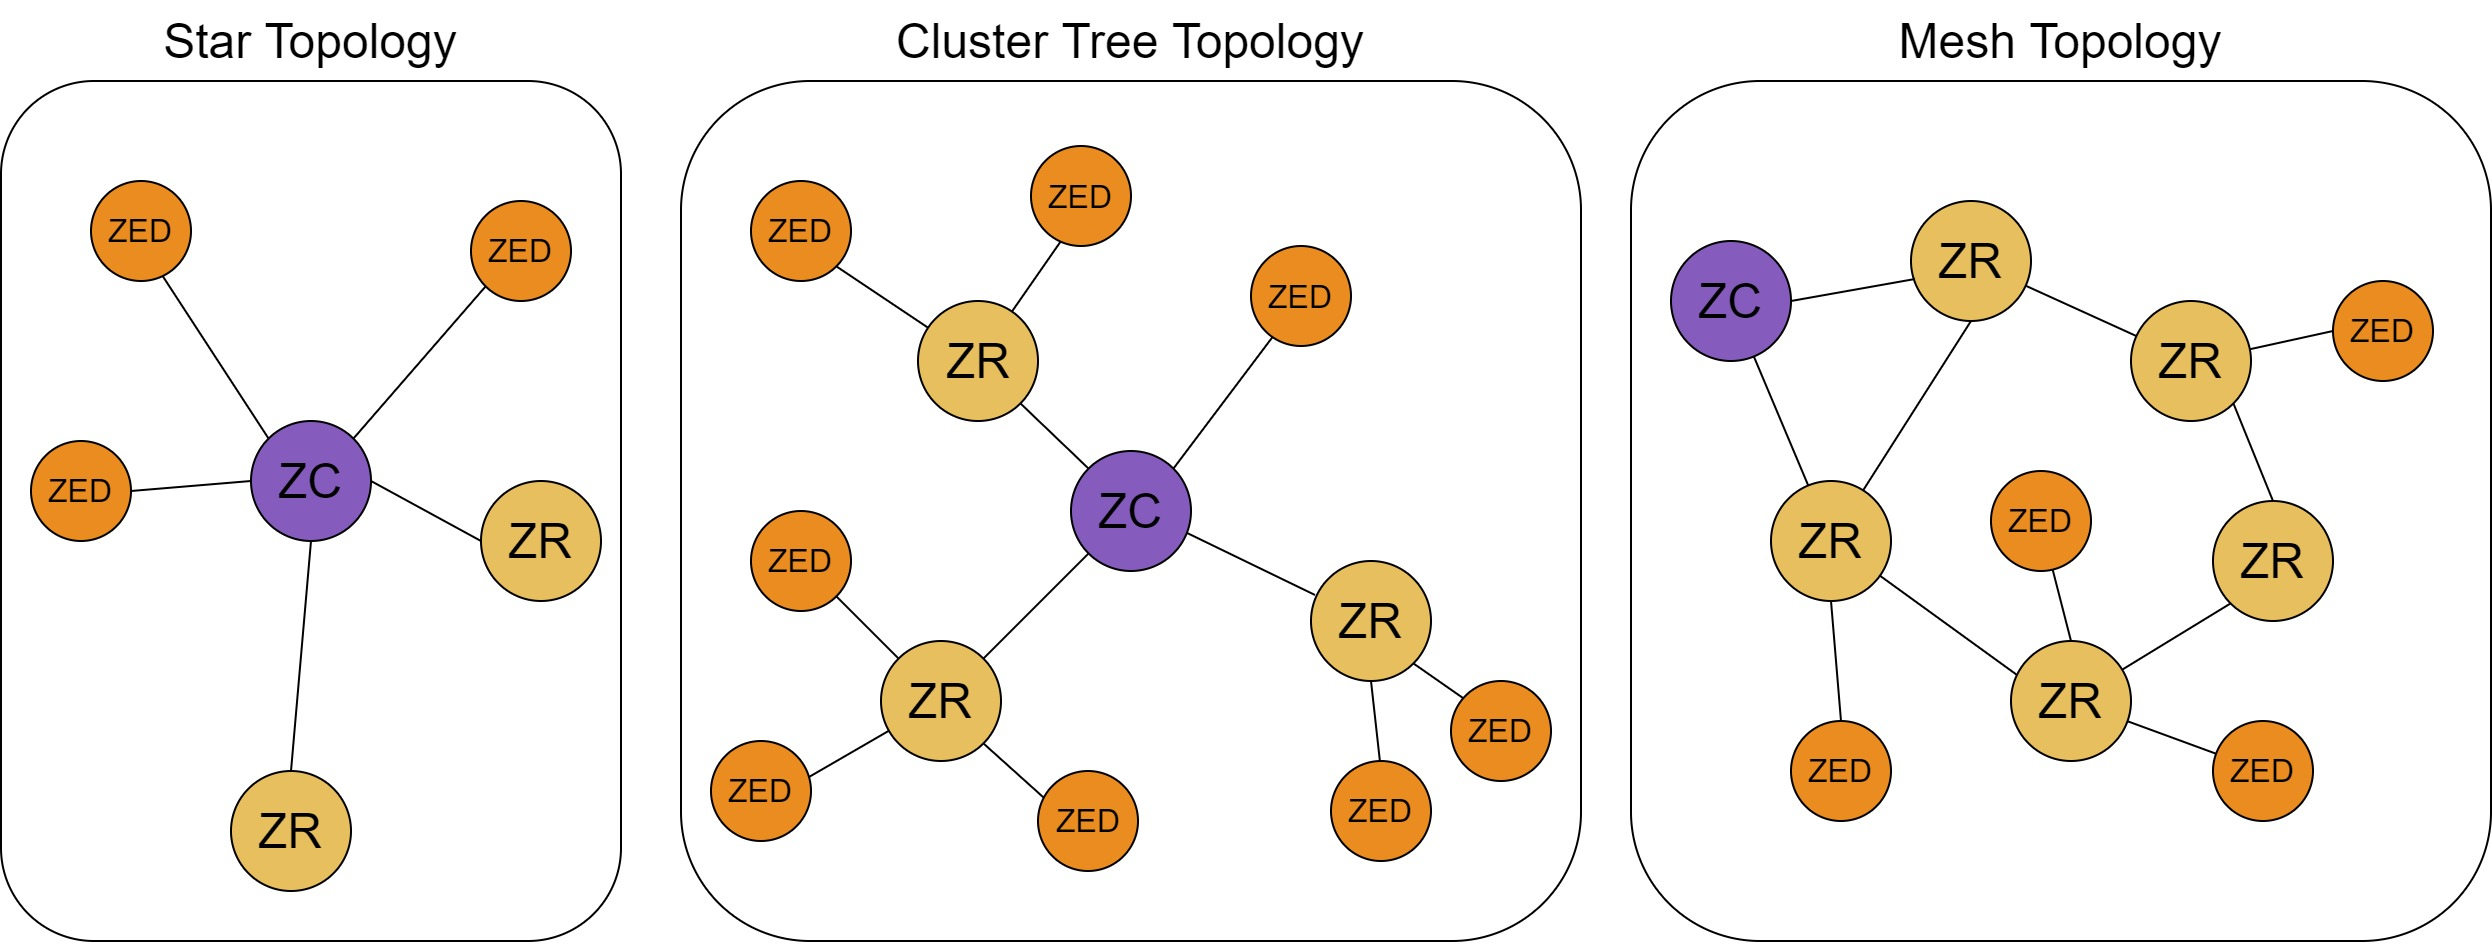
\includegraphics[width=1.0\textwidth]{./images/zigbee-arch.jpg}
  \end{center}
  \vspace{-5pt}
  \caption[Zigbee Netzwerkarchitekturen]{Zigbee Netzwerkarchitekturen}
  \caption*{Quelle: {\cite{IoTAndEdge.2020} (bearbeitet)}}
  \label{fig:zigbee-arch}
  \vspace{-10pt}
\end{figure}

Wie in Abbildung \ref{fig:zigbee-arch} dargestellt, unterstützt das Protokoll Zigbee drei verschiedene Netzwerk-Topologien: Star, Mesh und Cluster-Tree. In allen Topologien ist ein sogenannter \Fachbegriff{Zigbee Coordinator} nötig, der für die Kontrolle des Netzwerks zuständig ist, somit aber gleichzeitig einen Single Point of Failure darstellt, da es stets nur einen Coordinator pro Netzwerk geben kann. Neben dem Coordinator werden außerdem \Fachbegriff{Zigbee Router} benötigt, welche sowohl für das Routing zwischen den Endgeräten, als auch für das Eintreten neuer Endgeräte ins Netzwerk zuständig sind. In der Abbildung werden Coordinator als ZC, Router als ZR und Endgeräte als ZED dargestellt. Mit Zigbee sind Bandbreiten von bis zu 250 Kbits/s möglich, was verglichen zu anderen IoT-Protokollen im höheren Spektrum liegt. Die Reichweite liegt hierbei zwischen 75 und 100 Metern in Gebäuden oder bis zu 300 Metern Luftlinie. Ein Zigbee-Netzwerk ist zwar auf eine maximale Anzahl von 65000 Geräten beschränkt, in der Praxis wird das Limit jedoch bereits weit früher erreicht. Eines der größten Probleme von Zigbee ist der Stromverbrauch. Zwar können Endgeräte in einen Sleep-Modus schalten, um den Verbrauch zu senken, Router und der Coordinator müssen jedoch stets aktiv sein, um das Netzwerk permanent aufrecht zu erhalten. Somit ist es nicht praktikabel, ein Zigbee-Netzwerk über längere Zeiträume batteriebetrieben aufrecht zu erhalten, sofern das ein Anspruch an das Netzwerk sein sollte. Weitere Informationen über ZigBee können in den Artikeln \cite{Rani.2019}, \cite{Salman.2019}  und \cite{ZigBeeSpecification.2015} nachgelesen werden.

\subsubsection{BLE}
\label{sec:ThHi:ble}

Bluetooth ist eine Technologie, die schon seit Jahrzehnten sowohl für den klassischen Datenaustausch, als auch für Zwecke, die wie beispielsweise Audiostreaming eine hohe Bandbreite und große Datenpakete erfordern, genutzt wird. Für Szenarien, in denen ein niedriger Energieverbrauch essentiell wichtig ist, wie zum Beispiel beim Einsatz von batteriebetriebenen Sensoren, ist die Technologie also nicht geeignet. Das ursprünglich 2006 von Nokia entwickelte Protokoll \Fachbegriff{Wibree} ging 2009 in die Bluetooth-Version 4.0 als \Fachbegriff{Bluetooth Low Energy} ein und schafft Abhilfe für das oben genannte Problem. Im Vergleich zum klassischen Bluetooth überzeugt Bluetooth Low Energy, kurz BLE, durch etwa ein Zehntel des Energieverbrauchs und bis zu 15 mal geringeren Latenzen, wobei das Protokoll am besten für kleine Daten\-pakete geeignet ist. 

\begin{figure}[H]
  \vspace{10pt}
  \begin{center}
    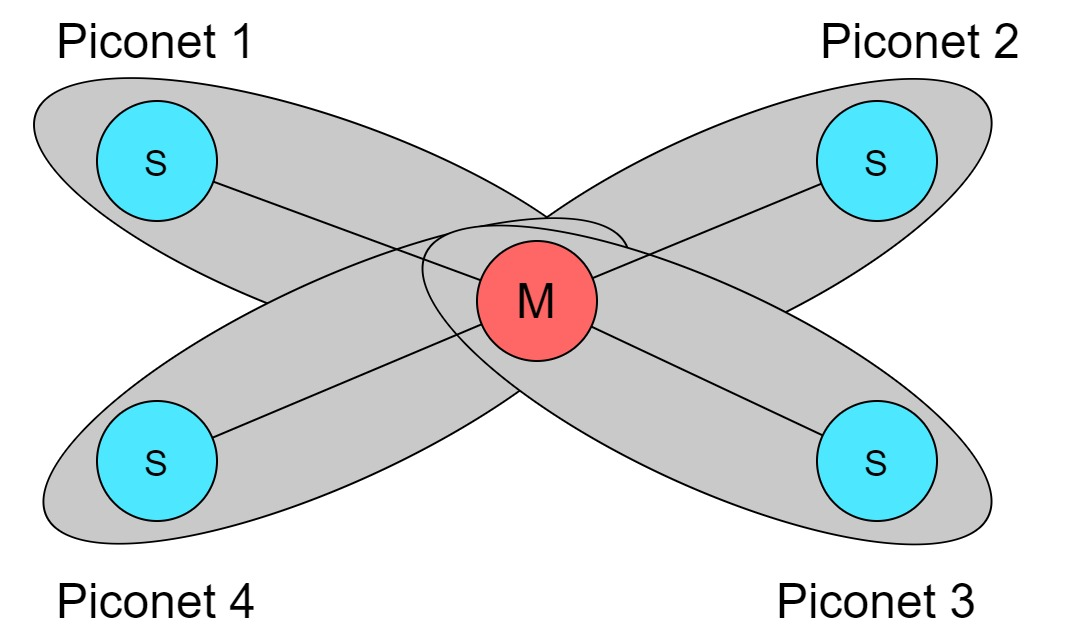
\includegraphics[width=0.6\textwidth]{./images/ble-pico.jpg}
  \end{center}
  \vspace{-5pt}
  \caption[BLE Master-Slave-Architektur]{BLE Master-Slave-Architektur}
  \caption*{Quelle: {\cite{IoTAndEdge.2020} (bearbeitet)}}
  \label{fig:ble-pico}
  \vspace{-10pt}
\end{figure}

Die Netzwerkarchitektur von BLE wird in Abbildung \ref{fig:ble-pico} dargestellt und stellt eine Master-Slave-Architektur dar. Jeder Slave baut hierbei eine Punkt-zu-Punkt-Verbindung zu einem Master auf und bildet ein sogenanntes \Fachbegriff{Piconet}. Mehrere Piconets können außerdem zu einem \Fachbegriff{Scatternet} zusammengeschlossen werden. Master-Nodes sind für die Kontrolle des Netzwerks, das Verbinden von neuen Nodes und die Synchronisation des Netzwerks zuständig. Endgeräte (Slaves) können bei Inaktivität in einen Sleep-Modus wechseln um Energie zu sparen, während Master-Nodes stets aktiv bleiben müssen. Aufgrund des niedrigen Energieverbrauchs und geringen Latenzzeiten wird BLE beispielsweise häufig in Kraftfahrzeugen zur internen Kommunikation von Geräten genutzt. Über Distanzen von etwa 100 Metern können mit Bitraten von bis zu 1 Mbit/s, beziehungsweise 2 Mbit/s bei der Verwendung von Bluetooth 5.0, Daten übertragen werden. Für die Verschlüsselung der Daten wird eine 128-Bit AES-Verschlüsselung genutzt, wobei im Vergleich zu Protokollen wie ZigBee eine eigene Verschlüsselung auf der Anwendungsschicht implementiert werden muss. Technische Details über Bluetooth und BLE können in der offiziellen Bluetooth Specification \Zitat{BluetoothSpecification.2015} gefunden werden, während der Artikel \cite{Salman.2019} einen Vergleich zu anderen Protokollen enthält.

\subsection{Low Power Wide Area Networks}
\label{sec:ThHi:lpwan}

Wie in Kapitel \ref{sec:ThHi:pan} bereits beschrieben wurde, müssen sich IoT-Lösungen, die auf WPAN-Techniken aufbauen, großen Herausforderungen stellen. Zum einen ist der Stromverbrauch der verwendeten Hardware oft sehr hoch, was den Batteriebetrieb von beispielsweise Türsensoren unpraktikabel macht. Zum anderen ist die Reichweite der Funkprotokolle für viele Szenarien mit großen Reichweitenanforderungen wie Smart Cities, oder oft sogar bereits für Smart Buildings nicht ausreichend. Dieser Punkt wird durch das Problem verstärkt, dass Funksignale durch Wände und ähnliche Hindernisse stark abgeschwächt und somit deren Reichweite weiter verringert wird. Für Usecases wie geografisches Tracking sind WPAN-Techniken aufgrund der Reichweite ebenfalls ungeeignet. Aus diesen Gründen steigt seit Jahren die Beliebtheit von LPWAN (Low-power Wide-area-networks) Techniken stark an. Es wird davon ausgegangen, dass im Jahr 2025 über 339 Millionen Geräte durch LPWAN-Techniken vernetzt sein werden \Zitat{Qihao.2019}. Protokolle dieser Klasse zeichnen sich primär durch sehr große Reichweiten aus. Ein nicht zu vernachlässigender Punkt ist außerdem, dass die Datenkommunikation mit sehr geringem Energieverbrauch funktioniert. Durch die hohe Reichweite ist die Bandbreite beim Datenversand geringer als bei WPAN-Techniken, wobei dies bei den normalerweise sehr kleinen IoT-Datenpaketen kein Problem darstellt. Die beliebtesten Netzwerktopologien sind Stern- und Meshtopologien. Meshnetzwerke bieten zwar einige Vorteile wie das Vorhandensein von mehreren Routen zum Nachrichtenversand (Redundanz), was beim Ausfall eines Empfängers Abhilfe schafft, und einfaches Skalieren des Netzwerks ermöglicht, jedoch werden Sterntopologien für LPWANs trotzdem bevorzugt. Dies liegt vor allem daran, dass Meshnetzwerke einerseits teurer sind und andererseits durch redundante Nodes einen deutlich höheren Energieverbrauch als Sterntopologien aufweisen \Zitat{Chaudhari.2020}. In diesem Abschnitt werden die Techniken \Fachbegriff{NB-IoT} und \Fachbegriff{Sigfox} thematisiert. 

\subsubsection{NB-IoT}
\label{sec:ThHi:nbiot}

Das 3rd Generation Partnership Project (3GPP) ist für die Standardisierung von Mobilfunktechniken wie LTE zuständig. Unter diese Standardisierungen fällt auch die 2016 veröffentlichte und für IoT-Zwecke optimierte Technologie \Fachbegriff{Narrowband Internet of Things}, kurz NB-IoT. Die Standardisierung macht es möglich, NB-IoT in das herkömmliche Mobilfunknetz zu integrieren, was einen immensen Vorteil darstellt, da dies die Vision in naher Zukunft ein global nutzbares IoT-Netzwerk zur Verfügung zu haben, sehr realistisch erscheinen lässt. Hier wird der große Vorteil gegenüber WPAN-Techniken klar: es existiert bereits ein Netzwerk, dessen (globale) Abde\-ckung von jedem genutzt werden kann. Dadurch werden Usecases wie Mobilität möglich, was bei WPAN-Technologien unmöglich ist. Eine 200-kHz-Funkzelle kann hierbei mehrere hunderttausend Geräte unterstützen. Der Name ``Narrowband IoT'' ergibt sich daher, dass das Protokoll zwar den LTE-Standard nutzt, sich jedoch auf eine schmale (englisch: narrow) Bandbreite von 200 kHz beschränkt. Zwar sinkt der Datendurchsatz gegenüber LTE, es steigt jedoch die Energieeffizienz und die Reichweite. Mit Geschwindigkeiten von bis zu 250 kb/s bei Downlink und bis zu 20 kb/s Uplink ist die Bandbreite für IoT-Zwecke jedoch weiterhin mehr als ausreichend. Das Nutzen des Mobilfunknetzes bietet immense Vorteile, wobei der größte die Quality of Service ist. Auch Geolokalisierung ist mit NB-IoT über TDoA (Time Difference of Arrival) möglich. Hierbei empfangen mehrere Funkmasten ein Signal gleichzeitig und können anhand der zeitlichen Unterschiede des Eintreffens der Signale den Sender lokalisieren. Das Senden von Daten geschieht über NB-IoT im Vergleich zu anderen LPWAN-Techniken mit hohen Geschwindigkeiten und niedrigen Latenzzeiten, wobei auch das Senden vieler Datenpakete kein Problem darstellt. Da NB-IoT im lizenzierten Spektrum operiert, gibt es hier keine Einschränkung über das Sendeverhalten von Geräten wie bei Protokollen wie Sigfox. Weitere Vorteile sind eine durch den Mobilfunk erprobte Ende-zu-Ende Verschlüsselung und Authentifizierung, hohe Skalierbarkeit, geringe Gerätekosten und eine gute Gebäudedurchdringung der Funksignale. Durch den niedrigen Energieverbrauch können NB-IoT-Geräte jahrelang batteriebetrieben genutzt werden. Dies macht es einfach, selbst komplexe IoT-Netzwerke aufzubauen, da Geräte weder zur Stromversorgung noch zum Datenaustausch verkabelt werden müssen. Jedoch gibt es auch Nachteile bei der Nutzung des Protokolls. Die Nutzung des Mobilfunknetzes ist bei der Nutzung von NB-IoT unabdingbar, es ist also nicht möglich eigene Netzwerke zu erstellen. Sollte beispielsweise die existierende Netz\-abdeckung für ein eigenes Szenario nicht ausreichend, oder ein vollständig privates Netzwerk erwünscht sein, ist NB-IoT für den Anwendungszweck ungeeignet. Außerdem verursacht die Nutzung des lizenzierten Spektrums Kosten, die vom Netzbetreiber festgelegt werden. Während hier nur ein Überblick über das Protokoll gegeben werden soll, beschäftigen sich die Artikel \cite{Aernouts.2018}, \cite{Vodafone.2017} und \cite{Ding.2020} noch detaillierter mit NB-IoT.

\subsubsection{Sigfox}
\label{sec:ThHi:sigfox}

Das französische Unternehmen \Begriff{Sigfox} wurde 2010 von Ludovic Le Moan und Christophe Fourtet mit der Vision gegründet, ein globales LPWA-Netzwerk aufzubauen. Im September 2020 gibt das Unternehmen an, über 16 Millionen Geräte, welche über 41 Millionen Nachrichten pro Tag senden, in 72 Ländern zu vernetzen. Sigfox bietet neben dem proprietären Funkprotokoll eine vollständige Ende-Zu-Ende-Konnektivität, wobei Geräte Daten über das Sigfox-Netzwerk direkt in die Sigfox-Cloud senden \Zitat{Sigfox.2020}. Sigfox operiert in den Frequenzbändern von 868 MHz in Europa, 902 MHz in den USA und 928 MHz in anderen Regionen, welche zum unlizenzierten Spektrum gehören und somit kostenfrei genutzt werden können. Sigfox nutzt in diesem Frequenzband nur 192 kHz und wird deswegen als ``Ultra-Narrow-Band'' bezeichnet. Mit einer Nachrichtenbreite von 100 Hz ist das Sigfox-Protokoll eines der Protokolle mit der schmalsten Bandbreite, wodurch geringe Geschwindigkeiten von bis zu 600 b/s beim Downlink und bis zu 100 b/s beim Uplink entstehen. Hierdurch entstehen im Umkehrschluss außerordentlich große Reichweiten von bis zu 50 Kilometern. Selbst Innenräume können durch das Sigfox-Netzwerk ausreichend abgedeckt werden.\\
Besonders vorteilhaft beim Protokoll Sigfox sind die geringen Kosten. Nutzer zahlen lediglich Sigfox-Nodes und die Kosten für die Nutzung des Netzwerks und der Sigfox-Cloud. Somit ist ein sehr einfaches Setup selbst von großen IoT-Netzwerken möglich, da die Geräteverwaltung und die Speicherung von Daten in einer Cloud ebenfalls Teil der Sigfox-Services ist und nicht selbst aufgesetzt werden muss. Geräte müssen mit Empfängerstationen keine stehende Verbindung halten, wodurch selbst mobile Geräte unterstützt werden. Sigfox-Nodes senden stets ein Paket direkt und zwei Kopien in einer zufälligen Frequenz an Stationen in Reichweite, was die Wahrscheinlichkeit für eine erfolgreiche Übermittlung deutlich erhöht. Die Daten werden hierbei vor dem Versand mit einer AES-Verschlüsselung versehen, um den Datenversand zwischen Gerät und Cloud komplett zu schützen. Die Netzwerktopologie von Sigfox wird als Sterntopologie bezeichnet, da jegliche Kommunikation im Netzwerk über Empfängerstationen (Sterne) des Netzwerks abläuft.\\
Die Nutzung von Sigfox bietet allerdings nicht nur Vorteile. Da Sigfox das gesamte Netzwerk bereitstellt, ist jeder Nutzer an das proprietäre Netzwerk gebunden. Dies ist vor allem deshalb ein Problem, da zum aktuellen Zeitpunkt zwar ein großer Teil Europas, andere Kontinente hingegen kaum durch das Sigfox-Netzwerk abgedeckt sind \Zitat{SigfoxMap.2020}. Somit kann ein Großteil der Welt Sigfox zum aktuellen Zeitpunkt nicht nutzen. Ein weiterer Nachteil ist eher technischer Natur. Sigfox-Nachrichten können lediglich mit 12 Bytes an Daten befüllt werden. Durch binäre Codierung können zwar für viele IoT-Szenarien ausreichend Daten verschickt werden, jedoch ist dies eine enorme Einschränkung gegenüber Protokollen wie NB-IoT. Ein Problem, dem sich alle LPWAN-Protokolle, die im unlizenzierten Spektrum agieren, stellen müssen, sind lokale Regulierungen, sogenannte \Begriff{Duty Cycles}. In Europa ist der Duty Cycle für das unlizenzierte Spektrum 1\%. Dies bedeutet, dass in einer Stunde, 3600 Sekunden, genau 1\% der Zeit gesendet werden darf, was 36 Sekunden entspricht. Da beim Uplink nach einer Nachricht mindestens 6 Sekunden gewartet werden muss, können also pro Gerät sechs Nachrichten pro Stunde, beziehungsweise 140 Nachrichten am Tag als Uplink gesendet werden. Somit ist Sigfox sehr ungeeignet für Szenarien in denen Echtzeitdaten oder eine hohe Nachrichtenanzahl erforderlich sind. Für Szenarien wie Smart Building oder Smart City hingegen ist Sigfox ideal, da die Datenmengen in derartigen Szenarien meist sehr gering und nicht zeitkritisch sind. Neben der offiziellen technischen Übersicht \Zitat{SigfoxTechnical.2017} wird Sigfox in den wissenschaftlichen Artikeln \cite{Aernouts.2018} und \cite{Chaudhari.2020} ausführlich behandelt.


\subsection{Messaging Protokolle}
\label{sec:ThHi:messaging}

Nachdem es Funkprotokolle möglich machen, Daten von Geräten wie Sensoren zu übertragen, müssen die Daten zur Weiterverarbeitung meist in einem System aus Services verbreitet werden. Ein Beispiel für eine solche Verbreitung ist das Hinterlegen eines empfangenen Datensatzes in die richtige Cloudinstanz, abhängig davon, welcher Nutzer hinter dem sendenden Gerät steht. Hierfür existieren diverse Protokolle, die nach dem TCP/IP-Schichtenmodell, anders als die bisher besprochenen Protokolle, der Anwendungsschicht zuzuordnen sind. Da die Anwendungsschicht auf die Netzwerkschicht und die Transportschicht aufbaut, sind derartige Protokolle für die Verbindung IoT-Geräte wie Sensoren zu Empfängern oft ungeeignet, da hierfür ein IP- und TCP-fähiges Netzwerk vorhanden sein muss. Aus diesem Grund werden in diesem Abschnitt kurz zwei Techniken beschrieben und die Frage geklärt, welche davon am besten geeignet ist und warum.

Das wohl älteste Protokoll hierfür ist das \Fachbegriff{Hypertext Transfer Protocol}, kurz HTTP. Das Protokoll baut auf TCP auf und garantiert somit einen erfolgreichen Nachrichtenversand, sowie Stau- und Flusskontrolle. Außerdem ist das Protokoll sehr einfach zu nutzen und auf den meisten Endgeräten implementiert. Trotzdem birgt die Nutzung des Protokolls immense Nachteile. Zum einen nutzt HTTP das Protokoll TCP der Transportschicht des TCP/IP-Modells. Um Nachrichten über TCP senden zu können, muss ein Three-Way-Handshake durchgeführt werden, der bei geringen Nachrichtengrößen, wie es bei IoT typisch der Fall ist, oft aufwendiger ist als das Senden der Daten an sich. Dadurch steigen die benötigten Ressourcen vor allem bei hohem Datendurchsatz stark an. Das Hauptproblem liegt aber in der Natur des HTTP Protokolls selbst. Es wird auf ein Request-Response-Format aufgebaut, was bedeutet, dass ein Sender eine Anfrage stellt und auf eine Antwort warten muss. HTTP wird daher auch als synchrones Protokoll bezeichnet. Dies ist nicht nur zeitaufwendig, sondern erfordert Ressourcen und blockiert eventuell andere Aufgaben. Zuletzt muss erwähnt werden, dass gerade bei der Verbreitung von Daten mit HTTP für jedes Ziel eine eigene Anfrage gestellt werden muss. HTTP scheint also allgemein für diesen Usecase nicht ideal geeignet zu sein \Zitat{Rani.2019}. 

Da das Request-Response-Format offensichtlich für IoT-Systeme eher ungeeignet ist, bauen die meisten modernen Systeme auf Publish-Subscribe-Formate auf. Das für Events optimierte Format besteht aus drei Komponenten: Publisher, Subscriber und Broker. Ein Publisher sendet hierbei Nachrichten an den Broker und versieht die Nachricht mit einer Annotation, dem sogenannten Topic. Subscriber können dem Broker vermitteln, an welchen Nachrichten sie interessiert sind. Hierfür geben die Subscriber ebenfalls ein oder mehrere Topics an. Es ist nun die Aufgabe des Brokers, eingehende Nachrichten an die passenden Subscriber zu verteilen. Hieraus ergeben sich große Vorteile. Zum einen sind Sender und Empfänger zeitlich nicht stark miteinander gekoppelt, es muss also nicht auf eine direkte Antwort gewartet werden. Diese Art von Protokollen kann daher als asynchron beschrieben werden. \\ 
Dies macht derartige Publish-Subscribe-Protokolle gerade für Netzwerke mit großen Latenzzeiten und niedrigen Bandbreiten geeignet, da der Nachrichtenversand keine blockierende Operation darstellt. Zum anderen werden Nachrichten nicht an einen speziellen Empfänger, sondern an eine symbolische Adresse, das Topic, gesendet. Dies macht es gerade in großen Systemen einfach, Nachrichten in einer Viele-zu-Viele-Beziehung zu verbreiten. Zudem ist der Inhalt der Nachrichten nicht an eine Programmiersprache gebunden, da für Sender und Empfänger lediglich das Kommunikationsformat festgelegt werden muss. Meist werden zwar die Formate JSON oder XML genutzt, jedoch kann theoretisch jedes beliebige Format genutzt werden. Das am häufigsten genutzte Protokoll dieser Art ist das \Fachbegriff{Message Queuing Telemetry Transport Protocol}, kurz MQTT. Das leichtgewichtige Protokoll fügt Nachrichten nur einen sehr schmalen Header von 2 Bytes hinzu, was Nachrichten allgemein sehr klein hält. Somit kann eine Vielzahl an Nachrichten verarbeitet werden, ohne die vorhandenen Ressourcen unnötig zu belasten. Neben der einfachen Nutzung des Protokolls existieren Client-Implementierungen für viele Programmiersprachen, was ebenfalls einen großen Vorteil von MQTT ausmacht. Aus diesen Gründen wird MQTT oft als Standard für IoT Messaging bezeichnet (\cite{Happ.2020, Rani.2019}). Weitere sehr beliebte und in vielen Punkten ähnliche Protokolle sind beispielsweise XMPP und AMQP.

\section{LoRa und LoRaWAN}
\label{sec:ThHi:loralorawan}

In diesem Kapitel wird das Protokoll LoRa, mit dem sich die Arbeit hauptsächlich beschäftigt, behandelt. Hierzu wird zunächst auf die Entstehungsgeschichte des Protokolls eingegangen. Daraufhin wird die Frage geklärt, worum es sich bei dem bereits erwähnten \Fachbegriff{LoRaWAN} handelt und welche Verbindung es zu LoRa hat. Ein großer Teil des Kapitels wird sich anschließend mit den technischen Details, der LoRaWAN Netzwerkarchitektur und der Sicherheit des Protokolls beschäftigen. Abschließend wird das ``The Things Network'' und das Unternehmen ``The Things Industries'' und deren Arbeit vorgestellt.

\subsection{Entstehung} 
\label{sec:ThHi:entstehung}

Die Geschichte von LoRa begann im Jahr 2009. Die beiden Franzosen Nicolas Sornin und Olivier Seller gründeten das Unternehmen \Begriff{Cycleo SAS} mit dem Ziel eine Technologie zu entwickeln, die es möglich macht, mit geringem Energieverbrauch Daten über große Distanzen zu übertragen. Hieraus ergibt sich auch der Name \Fachbegriff{LoRa}, welcher lediglich ein Akronym aus den englischen Worten ``Long Range'', also große Reichweite, darstellt. Da es zu dieser Zeit noch kaum vergleichbare Technologien gab, war dieses Protokoll ein revolutionärer Schritt in der IoT-Welt. Der dritte Partner François Sforza trat dem Unternehmen 2010 bei. Die ursprüngliche Zielgruppe von Gas-, Wasser- und Elektrizitätsmessung ähnelte bereits der Art von Vernetzung, die heute als ``Internet of Things'' bekannt ist. Im Mai 2012 kaufte die Firma \Begriff{Semtech} das Unternehmen auf und veröffentlichte das Protokoll \Fachbegriff{LoRaMAC}. Dieses neue Protokoll beinhaltete nicht nur die Datenübertragung durch Funksignale, sondern auch Eigenschaften wie Nachrichtenstandards und Sicherheit. Drei Jahre später, 2015, wurde die \Begriff{LoRa Alliance} gegründet, die bis heute das Ziel verfolgt, ihr Protokoll global nutzbar und Geräte miteinander kompatibel zu machen. Im gleichen Atemzug wurde das Protokoll zu \Fachbegriff{LoRaWAN} umbenannt \Zitat{Slats.2020}. Der Non-Profit-Organisation sind heute über 500 Unternehmen wie beispielsweise IBM und Cisco beigetreten, die alle das gemeinsame Ziel verfolgen, LoRaWAN als Standard für LPWA-Netzwerke nutzbar zu machen. Im November 2020 ist LoRaWAN in 162 Ländern vertreten und zählt somit zu den meist genutzten LPWAN-Technologien \Zitat{LoRaAlliance.2020}.

\subsection{Unterschied zwischen LoRa und LoRaWAN}
\label{sec:ThHi:lorawan}

Wichtig zu verstehen ist der Unterschied zwischen \Fachbegriff{LoRa} und \Fachbegriff{LoRaWAN}. LoRa stellt hierbei die erste, physikalische Schicht des TCP/IP-Schichtenmodells und ist somit lediglich für die Übertragung von Binärdaten zuständig. Für große Lösungen ist LoRa jedoch nicht ausreichend, da wichtige Eigenschaften wie Authentifizierung von Geräten oder eine einheitliche Netzwerkarchitektur nicht vorhanden sind. LoRaWAN ist ein cloudbasiertes Protokoll welches die Netzwerk\-schichten über LoRa abdeckt. Durch LoRaWAN werden, für LPWA-Netzwerke elementar wichtige, Funktionen wie Verschlüsselung und das Filtern duplizierter Nachrichten, bereitgestellt. Auch alle nötigen Netzwerk\-komponenten und deren Struktur werden durch LoRaWAN definiert. Um LoRa also optimal nutzen zu können, wird in beinahe allen Sze\-narien LoRaWAN ebenfalls verwendet. Besonders wichtig ist hierbei, dass LoRa selbst ein proprietäres Protokoll ist, während LoRaWAN ein völliges Open-Source-System darstellt \Zitat{LoRaAlliance.2015}.

\subsection{Technische Details}
\label{sec:ThHi:technisch}

LoRa und das damit verbundene Protokoll LoRaWAN sind in die Klasse der LPWA-Netzwerke in Kapitel \ref{sec:ThHi:lpwan} einzuordnen. Wie bereits erwähnt, stellt LoRa die physikalische Schicht im Netzwerkmodell dar. Protokolle dieser Schicht müssen stets mit Datenkollisionen kämpfen, die genau dann entstehen, wenn mehrere Sender über das gleiche Medium, zum Beispiel ein Ethernet-Kabel, senden. Um derartigen Kollisionen entgegen zu wirken, nutzt LoRa als erstes Protokoll die Modulationstechnik \Fachbegriff{Chirp Spread Spectrum}, kurz CSS, zum Datenversand. Hierbei handelt es sich um eine Technik, welche die Prinzipien mehrerer Modulationstechniken vereint, und somit besonders effektiv ist. Bei diesen Techniken handelt es sich um \Fachbegriff{Amplitude Modulation}, kurz AM, \Fachbegriff{Frequency Modulation}, kurz FM und \Fachbegriff{Phase Modulation}, kurz PM, wobei die ersten beiden Techniken beispielsweise aus dem Radiofunk bekannt sind. Das Ergebnis wird als \Fachbegriff{Multidimensional Multiple Access}, kurz MDMA bezeichnet. MDMA ist somit ausgesprochen robust und löst neben Datenkollisionen viele Probleme, die beim Datenversand mit Funktechniken entstehen können \Zitat{Bastani.2009}. 

Wie auch das in Kapitel \ref{sec:ThHi:sigfox} behandelte Protokoll Sigfox operiert LoRa im unlizenzierten Spektrum und kann somit kostenfrei privat genutzt werden. Die LoRa Alliance definiert diesen Frequenzbereich abhängig von der Region. In Europa wurde dieser beispielsweise auf 863-870 MHz (seltener auch 433-434 MHz) und in den USA auf 902-928 MHz festgelegt. Es gibt jedoch für jede Region eine Standardfrequenz, die beispielsweise für Anfragen zum Beitritt zum Netzwerk genutzt wird, woraufhin der gesamte Frequenzraum zur Verfügung steht. In Europa beträgt diese Frequenz 868 MHz, weshalb die Region auch oft als \Begriff{EU868} beschrieben wird. Ebenfalls ähnlich zu Sigfox existiert für LoRa eine weitere lokale Regulierung, der Duty Cycle. In Europa beträgt dieser meist 1\%, was eine Sendezeit von 36 Sekunden pro Stunde ergibt. Hierbei gibt es jedoch keine maximale Tagesanzahl an Nachrichten wie bei Sigfox, das Limit hängt lediglich von der genutzten Sendezeit und somit von der Sendedistanz und der Datenmenge ab. Da sich auch LoRaWAN-Empfangsstationen, sogenannte Gateways, an diesen Duty Cycle halten müssen, diese jedoch Nachrichten an mehr als nur ein Gerät senden können, wird in der LoRa-Kommunikation die Uplink-Richtung, also von Endgerät zu Gateway, stark präferiert. \\
Aus diesem Grund werden LoRa-Geräte in drei Klassen A, B und C eingeteilt. Jedes Gerät unterstützt hierbei die Klasse A. Diese ist die energiesparendste der Klassen, da sie sich auf Uplink nach der ALOHA-Methode verhält. Dies bedeutet, dass das Gerät Daten dann senden kann, wenn Sendebedarf besteht, und den Rest der Zeit in einem Energiesparmodus verweilen kann. Nach dem Datenversand folgen außerdem zwei kurze Zeitfenster, in welchen das Gerät Daten empfangen kann. Der Energieverbrauch ist hier so gering, dass viele Sensoren über mehrere Jahre rein batteriebetrieben im Einsatz bleiben können. Geräte der Klasse B folgen den Eigenschaften der vorherigen Klasse, jedoch mit dem Zusatz, dass die Geräte in bestimmten Zeitabständen aufwachen, um sich mit dem Netzwerk auszutauschen. Dies bietet den großen Vorteil, dass eine Garantie besteht, dass Daten mit einer bestimmten Verzögerung, die maximal die Aufwachfrequenz des Gerätes ist, an das Endgerät gesendet werden können. Diese Funktionalität macht sich jedoch im Energieverbrauch negativ bemerkbar. Abschließend folgen Geräte der Klasse C. Diese Geräte lauschen stets auf eingehende Nachrichten, sofern das Gerät selbst nicht sendet, weswegen die Geräte auch als halbduplexe Geräte bezeichnet werden können. Da im Gegensatz zu den Klassen A und B auf einen Energiesparmodus verzichtet wird, kostet diese Funktionalität offensichtlich deutlich mehr Energie, was die Geräte ungeeignet für batteriebetriebene Szenarien macht \Zitat{LoRaAlliance.2015}. 

Ein Aspekt, der LoRa stark von Sigfox unterscheidet, ist die Aufteilung des Frequenzraums in Kanäle. In Kombination mit der Nutzung des Chirp Spread Spectrums können somit Nachrichten gleichzeitig auf verschiedenen Kanälen gesendet werden, ohne Kollisionen zu verursachen \Zitat{LoRaAllianceRegional.2020}. In Europa beispielsweise definiert LoRaWAN 10 Kanäle mit einer variablen Datenrate von 250 b/s bis 5.5 kb/s, einen Kanal für schnelle Übertragungen mit bis zu 11 kb/s und einen FSK Kanal mit 50 kb/s, was die technisch höchste Datenrate von LoRaWAN darstellt \Zitat{LoRaAlliance.2015}. FSK steht hierbei für Frequency Shift Keying, worauf in dieser Arbeit jedoch nicht weiter eingegangen werden soll. Es gilt hier zu beachten, dass verschiedene Kanäle unterschiedliche Bandbreiten nutzen.

Zur Berechnung des tatsächlichen Datendurchsatzes müssen zwei weitere Konzepte verstanden werden. Zum einen ist das die sogenannte Coding Rate. Diese gibt an, wie groß der Teil eines LoRa-Pakets ist, der Daten beinhaltet, wobei der Rest des Pakets Metainformationen und ähnliches beinhaltet. Zum anderen kommt einer der wichtigsten Aspekte des LoRaWAN-Nachrichtenversands ins Spiel: der Spreading Factor, abgekürzt SF. Der Spreading Factor reicht von 7 bis 12, kann also 6 Werte annehmen. Je niedriger der Spreading Factor, desto höher die Datenrate. Es gilt jedoch zu beachten, dass sich die Sendereichweite indirekt proportional zum Spreading Factor verhält, also mit höherer Datenrate nur über geringere Reichweiten gesendet werden kann. Die SF-Auswahl hängt daher von der Entfernung zur Empfangsstation ab: befindet sich ein Endgerät nah am Empfänger, wird ein möglichst geringer SF gewählt, um durch das schnelle Senden der Nachricht mit einer hohen Datenrate das Netz nur einer möglichst geringen Belastung auszusetzen. Außerdem ist es durch verschiedene Spreading Factors ebenfalls möglich gleichzeitig Daten ohne Interferenzen zu senden, was gerade bei vielen verschiedenen Netzwerken in Kombination mit den anderen Modulationstechniken zu einem sehr robusten Sendeverhalten führt. 

Wie bei allen Funktechnologien ist es schwer, eine allgemeine Aussage über die tatsächliche maximale Sendereichweite, also mit dem höchsten Spreading Factor und der geringsten Datenrate, zu treffen. Viele Tests ergeben jedoch Distanzen von 2-5 Kilometern in städtischen Regionen und bis zu 30 Kilometern bei einer direkten Übertragung ohne Hindernisse \Zitat{Ertuerk.2019}. Somit ist es möglich mit wenigen Empfängerstationen ganze Städte abzudecken oder in Usecases wie Smart Buildings mit nur einem Gateway selbst Geräte in großen Gebäuden zu vernetzen.\\
Auch LoRaWAN ermöglicht es, einen Sender über den Zeitunterschied oder den Unterschied der Stärke der Signaleingänge zu orten, sollte das Signal von mehreren Empfangs\-stationen des gleichen Netzwerks empfangen werden. Durch die hohe Reichweite können also auch mobile Usecases verwirklicht werden.

Der wohl größte Vorteil gegenüber anderen LPWAN-Techniken, speziell der sehr ähnlichen Technologie Sigfox, ist die Möglichkeit eigene Netzwerke aufbauen zu können. Zwar ist die Anzahl der Nachrichten ähnlich wie bei Sigfox durch einen Duty Cycle limitiert, jedoch wird die maximale Nachrichtenanzahl nur durch die Uplink-Zeit, nicht aber durch Sendepausen wie bei Sigfox beeinflusst. Da LoRa im unlizen\-zierten Spektrum operiert, fallen für die Nutzung des Funkspektrums keinerlei Kosten an. Um ein eigenes Netzwerk aufzubauen, werden als Hardware lediglich ein LoRa-Gateway als Empfangsstation und LoRa-Endgeräte benötigt. Im Jahr 2020 existiert hierfür ein großer Markt, wodurch LoRa eine der günstigsten Techniken für ein eigenes LPWA-Netzwerk darstellt. Wie im Kapitel \ref{sec:ThHi:architektur} näher erläutert wird, können die Kosten für ein Gateway sogar vernachlässigt werden, wenn das Netzwerk eines externen Providers anstelle eines eigenen Netzwerks genutzt wird. Auch glo\-bale öffentliche Netzwerke sind mit LoRaWAN möglich, wobei eines davon in Kapitel \ref{sec:ThHi:ttntti} behandelt wird.


\subsection{LoRaWAN Netzwerkarchitektur} % Sicherheit nur kurz erwähnen, dann im nächsten Punkt
\label{sec:ThHi:architektur}

Die Softwareseite eines LoRaWAN-Netzwerks hingegen folgt im internen Aufbau der modernen Service-orientierten Architektur, kurz SOA. Im Gegensatz zu bis\-herigen Ansätzen werden Softwarefunktionalitäten in Services gruppiert und somit die mono\-lithische Applikation in mehrere kleine Applikationen aufgeteilt. Neben den typischen Vorteilen von SOAs gegenüber Monolithen bietet diese Struktur hier vor allem zwei große Vorteile. Wie im Kapitel \ref{sec:ThHi:sicherheit} weiter erklärt wird, werden Nachrichten, die durch den LoRaWAN-Stack gesendet werden, mehrfach verschlüsselt. Da es lediglich einen Service gibt, der sich mit dieser Verschlüsselung beschäftigt, senden die anderen Services (selbst das Gateway) die Daten lediglich weiter, ohne sie lesen zu können. Somit kann Vertrauen zu externen Netzwerkprovidern aufgebaut werden. Außerdem können die einzelnen Komponenten auf verschiedenen Geräten bereitgestellt werden. Dies dient nicht nur der Lastverteilung sondern gehört teilweise zur Funktionalität des LoRaWAN-Stacks. So wird beispielsweise der Service \Fachbegriff{Packet Forwarder} immer auf den LoRaWAN-Empfangsstationen, sogenannte Gateways, installiert.

Die Softwarekomponenten eines LoRaWAN-Netzwerkes sind der \Begriff{Packet Forwarder}, die \Begriff{Gateway Bridge}, der \Begriff{Join Server}, der \Begriff{Network Server} und der \Begriff{Application Server}. Auf die Aufgaben jeder Komponente wird nun intensiv eingegangen. Es gilt hier zu erwähnen, dass dies die typische LoRaWAN-Netzwerkarchitektur darstellt, und durchaus Abwandlungen dieses Aufbaus existieren. 

\begin{figure}[H]
  \vspace{10pt}
  \begin{center}
    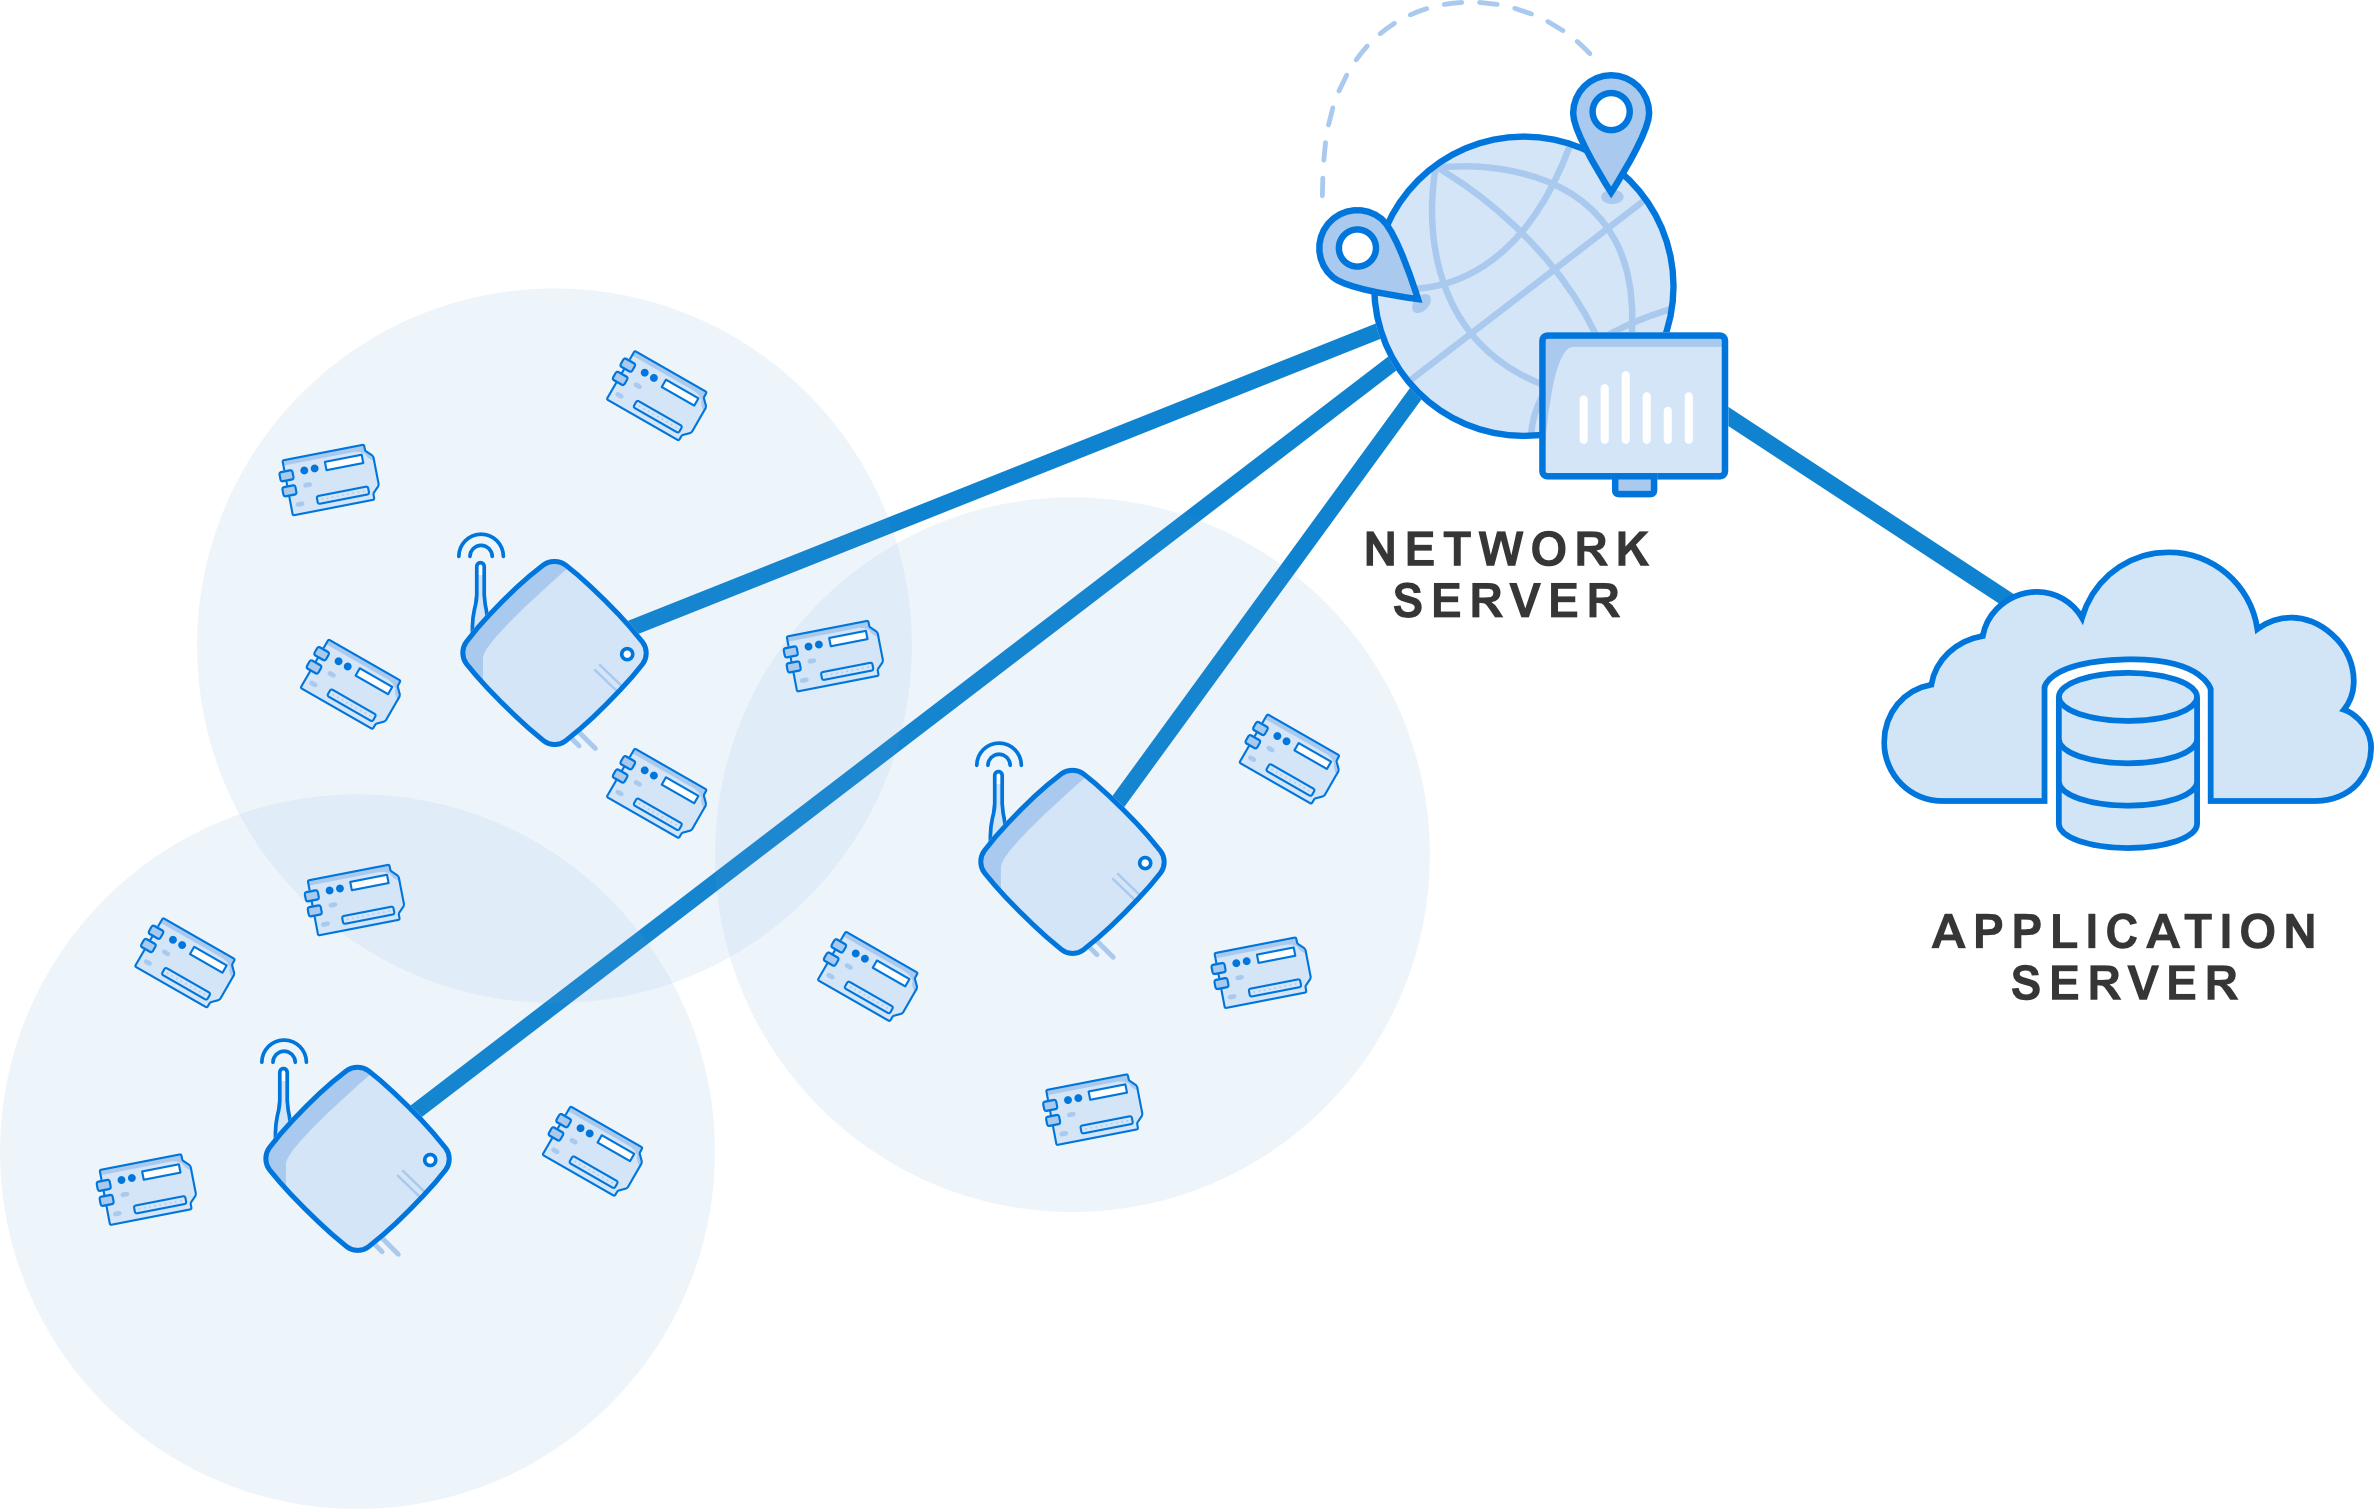
\includegraphics[width=0.7\textwidth]{./images/ttn-arch-star.jpg}
  \end{center}
  \vspace{-5pt}
  \caption[LoRaWAN Star-of-Stars-Topologie]{LoRaWAN Star-of-Stars-Topologie}
  \caption*{Quelle: {thethingsnetwork.org/docs/network/architecture.html}}
  \label{fig:ttn-arch-star}
  \vspace{-10pt}
\end{figure}

Wie aus Abbildung \ref{fig:ttn-arch-star} hervorgeht, stellt ein LoRaWAN-Netzwerk eine Star-of-Stars-Topologie dar, wobei der Network Server das Zentrum beziehungsweise der zentrale Stern der Topologie ist. Gateways stellen im Netzwerk die kleineren Sterne dar und leiten Nachrichten lediglich von den Endgeräten zum Network Server weiter. Außerdem wird hier der Begriff LoRaWAN statt LoRa verwendet, da es sich hier um die gesamte Netzwerkarchitektur und nicht nur um das Protokoll zum Datenversand vom Endgerät zum Empfänger handelt.

Wird ein Signal von einem LoRaWAN-Endgerät gesendet, wird dieses Signal als erstes von einem LoRaWAN-Gateway empfangen. Das Gateway hat eine der wichtigsten Aufgaben im Netzwerk: es dient als Proxy vom Endgerät in den LoRaWAN-Stack, welcher meist in cloudbasierten Lösungen lebt. Diese Funktionalität der Weiterleitung übernimmt der sogenannte Packet Forwarder. Dieser erfüllt also die relativ einfache Aufgabe, Nachrichten über LoRa zu empfangen und über ein IP-basiertes Protokoll, häufig UDP, weiter zu leiten.\\ Die meisten Gateways nutzen hierfür den von Semtech entwickelten \Fachbegriff{Semtech UDP Packet Forwarder}. Die Komponente ist die Minimalanforderung an installierter Software auf einem Gateway. Die verbleibenden Komponenten können theoretisch alle in der Cloud bereitgestellt werden. Per UDP werden die empfangenen Daten an die nächste Softwarekomponente, die Gateway Bridge, weitergeleitet.
Die Gateway Bridge hat die Aufgabe, das Format des Packet Forwarders in ein für den LoRaWAN-Stack normiertes Datenformat umzuwandeln, und die umgewandelten Daten weiterzuleiten. Hierbei sind die beliebtesten Formate \Fachbegriff{JSON} und Googles \Fachbegriff{Protobuf}. Weitergeleitet werden die Daten im neuen Format an einen Message Broker über ein Messaging Protokoll (siehe Kapitel \ref{sec:ThHi:messaging}) wie zum Beispiel MQTT. Die gesamte folgende netzwerkinterne Kommunikation geschieht also asynchron. Der Grund hierfür ist die Entlastung der einzelnen Komponenten: müsste die Gateway Bridge auf den erfolgreichen Versand und deren Antwort warten, und währenddessen blockieren, könnten andere Nachrichten verloren gehen. Somit können selbst Ausfälle einzelner Komponenten toleriert werden, da der Message Broker Daten zwischenspeichert und auch verspätet ausliefern kann.\\
Die Gateway Bridge kann entweder direkt auf dem Gateway oder mit den anderen Komponenten auf einem Server beispielsweise in der Cloud bereitgestellt werden. Für die Installation auf dem Gateway selbst spricht, dass MQTT über TCP läuft, und daher einen erfolgreichen Nachrichtenversand garantiert, während der Packet Forwarder UDP nutzt, welches verlorengegangene Nachrichten schlicht ignoriert. Außerdem ist es mit UDP nicht möglich eine verpflichtende Authentifizierung durchzuführen, da jeder das UDP Paket eines fremden Senders nachahmen und sich somit als dieser ausgeben kann. Mit MQTT besteht die Möglichkeit einer Authentifizierung, weswegen MQTT präferiert werden sollte. Meist wird die Gateway Bridge mit den verbleibenden Komponenten installiert, um sowohl Gateways mit, als auch Gateways ohne installierte Gateway Bridge unterstützen zu können. \\
Folgt man weiter dem Datenfluss, erreicht man nun den Network Server, das Herz der LoRaWAN Sterntopologie. Dieser bearbeitet nicht nur die meisten Aufgaben sondern ist für den Großteil der LoRaWAN-Funktionalität zuständig. Beachtet man vorerst nur den Datenfluss, ist die Hauptaufgabe des Network Servers Daten zwischen Gateways und der nächsten Komponente, dem Application Server, auszutauschen. Wurden die von den Endgeräten versendeten Daten von mehreren Gateways empfangen, ist es außerdem die Aufgabe des Network Servers, diese Duplikate zu erkennen und zu filtern. Hierbei werden Daten nicht direkt an den Network Server gesendet, da die vorherige Komponente, die Gateway Bridge, die Nachrichten bereits auf einem Message Broker hinterlegt hat. Wie in Kapitel \ref{sec:ThHi:messaging} erklärt, muss sich der Network Server also lediglich auf das passende Topic subscriben um die Nachrichten zu erhalten. \\
Die Aufgaben der Komponente betreffen aber nicht nur den Datenversand, sondern das gesamte Netz. Der Network Server ist beispielsweise für die Behandlung von Join Requests/Responses, also dem Beitritt neuer Geräte ins Netzwerk zuständig. Diese Verarbeitung solcher Requests und die Verschlüsselung der Nachrichten werden jedoch nicht vom Network Server selbst erledigt, sondern an den sogenannten \Fachbegriff{Join Server} delegiert. Außerdem steuert der Network Server die sogenannte \Fachbegriff{Adaptive Data Rate}, kurz ADR. Somit wird die Data Rate aller Geräte gesteuert, um beispielsweise Netzwerküberlastung zu vermeiden, beziehungsweise zu behandeln. Hat der Network Server beim Datenempfang all seine Arbeit geleistet, sendet er die verarbeiteten Daten wieder zum Message Broker. \\
Die letzte Komponente, die sich direkt mit dem Datenfluss beschäftigt, ist der Application Server. Auch diese Komponente ist für wichtige Aufgaben zuständig. Hierfür gilt es zu verstehen, dass der Application Server das Administrationswerkzeug eines LoRaWAN-Netzwerks darstellt. Über eine Weboberfläche kann das Netzwerk selbst verwaltet werden, also zum Beispiel neue Endgeräte oder Gateways registriert werden. Wird ein externer Netzwerkprovider genutzt, ist dies besonders wichtig, da nur durch diese Registrierung Daten vom Network Server an die richtige Adresse gelangen. Derartige Server bieten meist eine komfortable Nutzerverwaltung, um gemeinsam auf das eigene Netzwerk zugreifen zu können. Außerdem können zusammengehörige Endgeräte in Gruppen, sogenannte Applications, eingeteilt werden. Da über LoRaWAN versendete Daten meist binär enkodiert werden, um das Netzwerk durch geringere Datenmengen weniger zu belasten und selbst mehr Sendeflexibilität zu erreichen, bietet der Application Server die Möglichkeit, die Nachrichten beim Empfang mit sogenannten Decoder-Funktionen zu decodieren. Meist werden diese Funktionen vom Gerätehersteller mitgeliefert, diese können jedoch nach Belieben verändert oder sogar komplett selbst geschrieben werden. 

\begin{figure}[H]
  \vspace{10pt}
  \begin{center}
    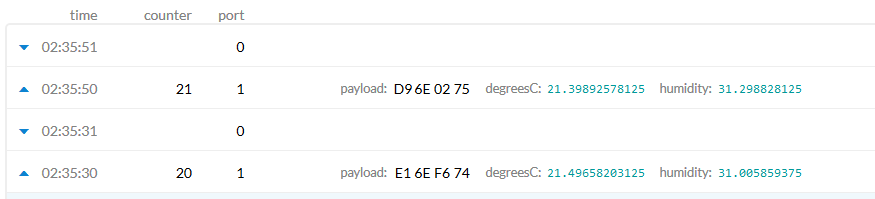
\includegraphics[width=1.0\textwidth]{./images/payload-decoding.png}
  \end{center}
  \vspace{-5pt}
  \caption[Payload Dekodierung]{Payload Dekodierung}
  \caption*{Quelle: {learn.adafruit.com/the-things-network-for-feather/payload-decoding}}
  \label{fig:payload-decoding}
  \vspace{-10pt}
\end{figure}

In Abbildung \ref{fig:payload-decoding} kann erkannt werden, wie aus einem binären Payload in hexadezimaler Schreibweise durch eine hinterlegte Decoder-Funktion ein Temperatur- und ein Luftfeuchtigkeitswert ausgelesen werden.

Neben der Organisation des Netzwerks wird der Application Server außerdem als API für IoT-Usecases wie beispielsweise der Datenvisualisierung genutzt. Hierfür bietet der Application Server APIs über Protokolle wie MQTT an, über die externe Clients die Daten selbst beziehen können. Auch sogenannte Integrations sind eine beliebte Möglichkeit, Daten weiterzuverarbeiten. Mit Integrations können empfangene Daten direkt vom Application Server weiterverarbeitet werden. Die InfluxDB-Integration, welche von vielen Application Servers implementiert wird, kann beispielsweise Messwerte direkt in eine Datenbank schreiben. \\
Über den Application Server können auch Daten an Endgeräte gesendet werden, was oft aus Konfigurations\-zwecken notwendig ist, da bei vielen Geräten keine Möglichkeit besteht, direkt auf die Software zuzugreifen, um diese zu konfigurieren.
Für die Netzwerksicherheit ist der bereits erwähnte Join Server zuständig. Je nach Implementierung ist dieser entweder wie beim \Fachbegriff{The Things Network} als separater Service bereitgestellt oder wie beim \Fachbegriff{ChirpStack} in einer Komponente, in diesem Fall im Application Server, integriert. Wichtig hierbei ist, dass der Network Server keine Kontrolle über die Verschlüsselung hat und somit der Betreiber des Netzwerks keinerlei fremde Nachrichten lesen kann. Auf die Funktionsweise der Verschlüsselung wird im Kapitel \ref{sec:ThHi:sicherheit} näher eingegangen. Bei der Recherche für dieses Kapitel wurden die Quellen \cite{TTNArch.2020}, \cite{ChirpArch.2020} und \cite{TTSApp.2020} hinzugezogen.


\subsection{Sicherheit}
\label{sec:ThHi:sicherheit}

LoRaWAN legt einen sehr hohen Wert auf die Sicherheit des Nachrichtenversands und nutzt eine 128-bit AES-Verschlüsselung. Jedes Endgerät wird vom Hersteller mit drei Keys ausgeliefert. Diese Keys sind eine \Fachbegriff{64-Bit-DevEUI}, eine \Fachbegriff{64-Bit-AppEUI} und ein \Fachbegriff{128-Bit-AppKey}, wobei EUI jeweils für Extended Unique Identifier steht. Diese Keys werden dann benötigt, wenn ein Gerät versucht, dem Netzwerk beizutreten. Beim erfolgreichen Netzwerkbeitritt werden zwei 128-bit Schlüssel generiert, der \Fachbegriff{NwkSKey} (Network Session Key) und der \Fachbegriff{AppSKey} (Application Session Key), wobei beide Schlüssel für nur dieses Gerät und diese Session genutzt werden. Verlässt ein Gerät das Netzwerk und tritt erneut bei, werden also zwei neue Schlüssel generiert. Wie später näher beschrieben wird, weicht dies jedoch bei der Aktivierungsmethode ``Activation by personalization'' ab. Sobald die Geräte beigetreten sind, werden alle Nachrichten zwischen dem Netzwerk und dem neuen Gerät mithilfe dieser beiden Schlüssel verschlüsselt. Der NwkSKey wird nach der Generierung zwischen dem Endgerät und dem Network Server geteilt und ist für deren sichere Kommunikation zuständig. Außerdem ist es durch den Schlüssel möglich, Nachrichten über eine Prüfsumme zu validieren, beziehungsweise Veränderungen festzustellen. Der AppSKey hingegen wird nur zwischen dem Endgerät und dem Application Server ausgetauscht. Dieser Key erlaubt es, Nachrichten Ende-zu-Ende zu verschlüsseln und zu versenden, sodass Komponenten wie der Network Server den Inhalt der Nachrichten nicht verstehen können. Dies ist besonders dann wichtig, wenn ein externer Netzwerkanbieter statt eines privaten Netzwerks genutzt wird, da hierdurch für diesen keine Möglichkeit besteht, Daten, die über sein Netzwerk versendet werden, zu lesen. Wie man also sieht, bietet LoRaWAN sowohl Sicherheitsvorkehrungen auf der Netzwerk-, als auch auf der Anwendungsebene.

Wie funktioniert jedoch der Beitritt zum Netzwerk? Allgemein werden neue Geräte vorerst im Application Server registriert, denn erst wenn das Gerät registriert ist, kann eine Join Request, also eine Anfrage, dem Netzwerk beizutreten, gestellt werden. Bei der Registrierung werden die bereits erwähnten Schlüssel des Endgeräts, nämlich die global eindeutige DevEUI, die AppEUI und der AppKey hinterlegt und außerdem die Aktivierungsmethode gewählt. Hierfür gibt es zwei verschie\-dene Methoden: \Fachbegriff{Over-The-Air-Activation (OTAA)} und \Fachbegriff{Activation-By-Personalization (ABP)}. OTAA stellt die Standardaktivierungsmethode für Endgeräte dar und ist die sicherere der beiden Methoden. Hier sendet ein Endgerät eine Join Request bestehend aus 4 Werten an den Network Server. Diese Werte sind die DevEUI, die AppEUI, die DevNonce und der Message Integrity Code, kurz MIC. Die DevNonce stellt hierbei eine zufällig generierte Zahl dar, die vor Angriffen auf den Aktivierungsprozess schützen soll. Der MIC wird für die Validierung der Nachricht wie auch beim späteren Nachrichtenversand genutzt. Wie oben erwähnt, werden bei einer validen Join Request nun der NwkSKey und der AppSKey mithilfe der Daten in der Join Request generiert. Der Network Server antwortet in einer Join Response mit einigen Werten, wobei der wichtigste die DevAddr ist. Die DevAddr ist eine netzwerkinterne, eindeutige Adresse, die für das neue Endgerät generiert wurde. Von nun an können das Endgerät und der Network Server verschlüsselt kommunizieren. Bei der alternativen ABP-Methode sind die DevAddr, der NwkSKey und der AppSKey bereits an das Gerät gebunden, es müssen also keine Schlüssel oder andere Werte generiert werden. Daher kann ein Netzwerkbeitritt ohne Join-Prozedur ablaufen. Der große Unterschied zwischen den Methoden ist daher, dass OTAA Keys, welche die gesamte Verschlüsselung von LoRaWAN steuern, für jede Session, also jede Registrierung eines Geräts neu generiert, während sich Keys bei ABP ohne manuelles Überschreiben nie ändern. Somit bietet ABP mehr Angriffsmöglichkeiten als OTAA und wird daher seltener verwendet. Zusammenfassend lässt sich sagen, dass LoRaWAN die bereits sehr umfangreiche Netzwerksicherheit auf bewährten Techniken wie AES aufbaut und auch weiterhin die Sicherheit eines LoRaWAN-Netzes durch regel\-mäßige Updates verbessert wird. Die Informationen dieses Kapitels stammen aus den Artikeln \cite{TTNSec.2020} und \cite{SmartMakers.2018}.


\subsection{The Things Network und The Things Industries}
\label{sec:ThHi:ttntti}

In dieser Arbeit wurden bereits mehrfach externe Netzwerkprovider erwähnt. Beschäftigt man sich mit LoRa und LoRaWAN, so stößt man früher oder später auf die Begriffe ``The Things Network'' und ``The Things Industries''. In diesem Kapitel wird erläutert, worum es sich bei den Begriffen handelt und wofür diese nützlich sind.

Bei dem The Things Network, kurz TTN, handelt es sich um ein völlig öffentliches LoRaWAN-Netzwerk. Unter öffentlich versteht man hierbei, dass es jedem möglich ist, Nachrichten über ebenfalls öffentliche Gateways zu senden. Zwar können mit eigenen Gateways und weiterer Hardware eigene ``The Things Network''-Netzwerke aufgebaut werden, da das TTN vollständig Open Source ist, jedoch ist es erwünscht, dem existierenden, kollaborativen Netzwerk beizutreten und dieses somit immer weiter zu vergrößern. Hierbei gilt es zu erwähnen, dass das The Things Network Forum aufgrund der riesigen Community eine der besten Ressourcen für LoRaWAN ist, in der viele Experten ihre Erfahrungen teilen oder auf Fragen antworten. Durch die große Community steigt jedoch nicht nur der Wissensaustausch, sondern auch die Netzwerkgröße. Die mittlerweile fast 16 000 Gateways in 150 Ländern im öffentlichen Netzwerk leiten LoRa-Nachrichten an den cloudbasierten Network Server weiter. Über die TTN-Console, welche ein User Interface zum, ebenfalls cloud\-basierten, Application Server darstellt, können Gateways und Endgeräte ins Netzwerk aufgenommen werden. Auch die anderen in Kapitel \ref{sec:ThHi:architektur} genannten Komponenten sind im The Things Network meist in der Cloud vertreten, wobei der gesamte Softwarestack auch als ``The Things Stack'' bezeichnet wird. Die einzige neue Komponente ist der \Fachbegriff{Identity Server}, der für die Zuordnung von Ressourcen im Netzwerk zu Nutzern und deren Verwaltung zuständig ist. Eine weitere Neuheit ist das \Fachbegriff{Gateway Connector Protocol}. Das Protokoll ersetzt das UDP-Protokoll in der Kommunikation zwischen Gateway und Network Server und löst wichtige Probleme wie den Mangel einer Authentifizierung oder einer Verschlüsselung die Veränderung der gesendeten Daten erkennt und behebt. Mit diesem Protokoll können Daten dann entweder per gRPC oder MQTT an den Network Server gesendet werden \Zitat{TTNGwConn.2020}.

Denkt man über ein öffentliches LoRaWAN-Netzwerk nach, werden schnell viele Vorteile klar. Ist ein Nutzer in Reichweite eines der öffentlichen Gateways, ist es ihm mit dem TTN möglich, LoRa-Geräte zu registrieren und zu nutzen, ohne selbst ein Gateway einrichten zu müssen. Existierende Gateways können hierbei über eine Karte eingesehen werden. 

\begin{figure}[H]
  \begin{center}
    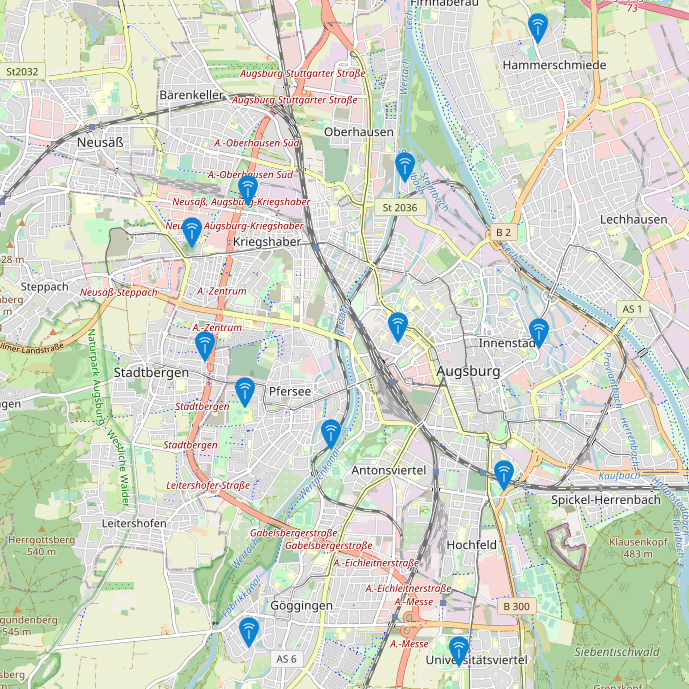
\includegraphics[width=0.65\textwidth]{./images/augsburg-coverage.png}  
    \end{center}
  \vspace{-5pt}
  \caption[The Things Network Gateways: Augsburg]{The Things Network Gateways: Augsburg}
  \caption*{Quelle: {thethingsnetwork.org/map}}
  \label{fig:augsburg-coverage}
  \vspace{-5pt}
\end{figure}

Da viele Städte bereits eine vollständige TTN-Abdeck\-ung vorweisen, können dort große IoT-Szenarien wie Smart Cities oder GPS-Tracking von Fahrrädern realisiert werden, ohne auf die Reichweite eigener Gateways limitiert zu sein. Abbildung \ref{fig:augsburg-coverage} zeigt die vorhandenen Gateways des The Things Network in der Stadt Augsburg im Dezember 2020. Der Ausschnitt der Karte zeigt in etwa 100 $km^2$ Fläche. Es kann davon ausgegangen werden, dass der Großteil der gezeigten Fläche durch die vorhandenen Gateways abgedeckt wird.

Die hohe Anzahl an Gateways und die cloudbasierten Netzwerkkomponenten sorgen außerdem für eine hohe Skalierbarkeit des Netzwerks. Das öffentliche Netzwerk kommt jedoch nicht ohne Nachteile gegenüber eines privaten Netzwerks aus. Der technisch interessanteste ist hierbei die sogenannte \Fachbegriff{Fair Use Policy}. Diese limitiert die erlaubte Nachrichtenanzahl über die lokalen LoRa-Regulierungen hinweg pro Gerät auf 30 Sekunden Uplink und 10 Nachrichten Downlink pro Tag \Zitat{TTN.2020}. Da öffentliche Gateways privat eingesetzt werden gibt es außerdem keine Garantie, dass diese durchgehend verfügbar sind, wodurch ein eigenes Gateway für wichtige Szenarien von essentieller Bedeutung sein kann.

Offensichtlich benötigt ein Netzwerk derartiger Größe ein hohes Maß an Standardisierung der genutzten Software und vor allem der Geräte. Daher wurde von den Entwicklern des The Things Network das Unternehmen The Things Industries gegründet, mit dem Ziel, ein LoRaWAN-Netzwerk mit tatsächlicher globaler Abde\-ckung aufzubauen. Das Unternehmen will dies erreichen, indem es eine ``integrierte Kette aus Produkten und Services'' für die Arbeit mit dem The Things Network bereitstellt. Das einfachste Beispiel hierfür sind die hauseigenen LoRaWAN-Gateways. Diese Gateways werden vorkonfiguriert geliefert und müssen für die Integration in das The Things Network lediglich mit Strom versorgt und in ein IP-basiertes Netzwerk aufgenommen werden. So fällt es Nutzern leicht mit dem Netzwerk zu inter\-agieren, ohne sich mit aufwendigen Konfigurationsarbeiten beschäftigen zu müssen.

Allgemein ist die Nutzung des The Things Network mit der Hardware von The Things Industries die wohl einfachste Möglichkeit des Einstiegs in die Thematik rund um LoRaWAN. The Things Industries bietet jedoch nicht nur Hardware als Produkte an. Da das The Things Network durch die Fair Use Policy gerade für große, kommerzielle Netzwerke oft nicht ausreichend ist, bietet das Unternehmen neben Consulting auch eigene, vollständig gehostete Deployments des The Things Stacks an \Zitat{TTI.2020}. Diese Art von Produkt wird auch als ``Software-as-a-Service'' bezeichnet. Innerhalb des eigenen Netzwerks kann der jeweilige Kunde dann frei agieren und muss lediglich die lokalen LoRa-Regulierungen wie den Duty Cycle (siehe Kapitel \ref{sec:ThHi:technisch}) einhalten.